\documentclass[10pt]{beamer}

% Beamer style
%\usetheme[secheader]{Madrid}
% \usetheme{CambridgeUS}
\useoutertheme{infolines}
\usecolortheme[rgb={0.65,0.15,0.25}]{structure}
% \usefonttheme[onlymath]{serif}
\beamertemplatenavigationsymbolsempty
%\AtBeginSubsection

% Packages
%\usepackage[french]{babel}
\usepackage[latin1]{inputenc}
\usepackage{color}
\usepackage{xspace}
%\usepackage{dsfont, stmaryrd}
\usepackage{amsmath, amsfonts, amssymb}
\usepackage{url}
\usepackage{./astats}
%\usepackage[all]{xy}
\usepackage{graphicx}
\usepackage{tikz}
\newcommand{\nodesize}{2em}
\newcommand{\edgeunit}{1*\nodesize}
\tikzstyle{node}=[point, inner sep=0]
\tikzstyle{edge}=[-, line width=.5pt]

% Not numbering backup slides
\newcommand{\backupbegin}{
   \newcounter{finalframe}
   \setcounter{finalframe}{\value{framenumber}}
}
\newcommand{\backupend}{
   \setcounter{framenumber}{\value{finalframe}}
}


% Commands
\definecolor{darkred}{rgb}{0.65,0.15,0.25}
\newcommand{\emphase}[1]{\textcolor{darkred}{#1}}
% \newcommand{\emphase}[1]{{#1}}
\newcommand{\paragraph}[1]{\textcolor{darkred}{#1}}
\newcommand{\refer}[1]{{\footnotesize{\textcolor{blue}{[{\cite{#1}}]}}}}
\newcommand{\Refer}[1]{{\footnotesize{\textcolor{blue}{[{#1}]}}}}
\renewcommand{\newblock}{}

% Symbols
\newcommand{\Abf}{{\bf A}}
\newcommand{\Beta}{\text{B}}
\newcommand{\Bcal}{\mathcal{B}}
\newcommand{\BIC}{\text{BIC}}
\newcommand{\Ccal}{\mathcal{C}}
\newcommand{\dd}{\text{~d}}
\newcommand{\dbf}{{\bf d}}
\newcommand{\Dcal}{\mathcal{D}}
\newcommand{\Esp}{\mathbb{E}}
\newcommand{\Espt}{\widetilde{\Esp}}
\newcommand{\Ebf}{{\bf E}}
\newcommand{\Ecal}{\mathcal{E}}
\newcommand{\Gcal}{\mathcal{G}}
\newcommand{\Gam}{\mathcal{G}\text{am}}
\newcommand{\Hcal}{\mathcal{H}}
\newcommand{\Ibb}{\mathbb{I}}
\newcommand{\Ibf}{{\bf I}}
\newcommand{\ICL}{\text{ICL}}
\newcommand{\Cov}{\mathbb{C}\text{ov}}
\newcommand{\Corr}{\mathbb{C}\text{orr}}
\newcommand{\Var}{\mathbb{V}}
\newcommand{\Vsf}{\mathsf{V}}
\newcommand{\pen}{\text{pen}}
\newcommand{\pt}{\widetilde{p}}
\newcommand{\Fcal}{\mathcal{F}}
\newcommand{\Hbf}{{\bf H}}
\newcommand{\Jcal}{\mathcal{J}}
\newcommand{\Kbf}{{\bf K}}
\newcommand{\Lcal}{\mathcal{L}}
\newcommand{\Mcal}{\mathcal{M}}
\newcommand{\mbf}{{\bf m}}
\newcommand{\mum}{\mu(\mbf)}
\newcommand{\Ncal}{\mathcal{N}}
\newcommand{\Nbf}{{\bf N}}
\newcommand{\Nm}{N(\mbf)}
\newcommand{\Ocal}{\mathcal{O}}
\newcommand{\Obf}{{\bf 0}}
\newcommand{\Omegas}{\underset{s}{\Omega}}
\newcommand{\Pbf}{{\bf P}}
\newcommand{\Pt}{\widetilde{P}}
\newcommand{\Pcal}{\mathcal{P}}
\newcommand{\Qcal}{\mathcal{Q}}
\newcommand{\Rbb}{\mathbb{R}}
\newcommand{\Rcal}{\mathcal{R}}
\newcommand{\Scal}{\mathcal{S}}
\newcommand{\Ucal}{\mathcal{U}}
\newcommand{\Vcal}{\mathcal{V}}
\newcommand{\BP}{\text{BP}}
\newcommand{\EM}{\text{EM}}
\newcommand{\VEM}{\text{VEM}}
\newcommand{\VBEM}{\text{VBEM}}
\newcommand{\cst}{\text{cst}}
\newcommand{\obs}{\text{obs}}
\newcommand{\ra}{\emphase{\mathversion{bold}{$\rightarrow$}~}}
%\newcommand{\transp}{\text{{\tiny $\top$}}}
\newcommand{\transp}{\text{{\tiny \mathversion{bold}{$\top$}}}}
\newcommand{\logit}{\text{logit}\xspace}

% Directory
\newcommand{\figmixt}{/home/robin/ENSEIGN/COURS/MELANGE}
\newcommand{\figbma}{/home/robin/RECHERCHE/RUPTURES/MELANGE/Exemples/Grippe}
\newcommand{\fignet}{../FIGURES}
\newcommand{\figeco}{/home/robin/RECHERCHE/ECOLOGIE/EXPOSES/FIGURES}
%\newcommand{\figmotif}{/home/robin/RECHERCHE/RESEAUX/Motifs/FIGURES}


%====================================================================
%====================================================================

%====================================================================
%====================================================================
\begin{document}
%====================================================================
%====================================================================

%====================================================================
\title[GOF for graph models]{Goodness of fit of logistic models for random graphs: \\
a variational Bayes approach}

\author[S. Robin]{S. Robin \\ ~\\
  Joint work with P. Latouche and S. Ouadah}

\institute[INRA / AgroParisTech]{INRA / AgroParisTech \\ ~\\
  \vspace{-.1\textwidth}
  \begin{tabular}{ccccc}
%     
\includegraphics[height=.3\textheight]{\fignet/LogoINRA-Couleur} & 
%     \hspace{.02\textheight} &
%     
\includegraphics[height=.08\textheight]{\fignet/logagroptechsolo} & 
%     \hspace{.02\textheight} &
%     
\includegraphics[height=.09\textheight]{\fignet/logo-ssb}
    
\includegraphics[height=.2\textheight]{\fignet/LogoINRA-Couleur} & 
    \hspace{.02\textheight} &
    
\includegraphics[height=.067\textheight]{\fignet/logagroptechsolo} & 
    \hspace{.02\textheight} &
    
\includegraphics[height=.06\textheight]{\fignet/logo-ssb}
    \\ 
  \end{tabular} \\
  \bigskip
  }

\date[MIAT, Nov. 2016]{MIAT Seminar, Toulouse, November 2016}

%====================================================================
%====================================================================
\maketitle
%====================================================================

%====================================================================
%====================================================================
\section*{Problem}
%====================================================================
\frame{ \frametitle{Motivating example}

  \begin{tabular}{cc}
%     \hspace{-.05\textwidth}
    \begin{tabular}{p{.4\textwidth}}
      \paragraph{Data:} $n=51$ tree species, \\
      $Y_{ij} =$ number of common parasites %\\
      \refer{VPD08}.

      \onslide+<2->{
        \bigskip
        \paragraph{Valued stochastic block model.} \\
        If $i \in \Ccal_k$, $j \in \Ccal_\ell$:
        $$
        Y_{ij} \sim \Pcal(\lambda_{k\ell}),
        $$
        $\lambda_{k\ell} =$ mean number of shared parasites.
        
        \bigskip
        \paragraph{Pseudo-BIC:} $K=7$ groups}
%       \onslide+<3->{
%         that are \emphase{strongly related with phylums}. 
%         }
      \end{tabular}
    & 
    \hspace{-.1\textwidth}
    \begin{tabular}{c}
      \onslide+<2->{
        {\tiny
          \begin{tabular}{c|ccccccc}
            $\widehat{\lambda}_{k\ell}$ & T1 & T2 & T3 & T4 & T5 & T6 &
            T7 \\ 
            \hline \hline
            T1 & 14.46 & 4.19 & 5.99 & 7.67 & 2.44 & 0.13 & 1.43 \\
            T2 &  & 14.13 & 0.68 & 2.79 & 4.84 & 0.53 & 1.54 \\
            T3 &  &  & 3.19 & 4.10 & 0.66 & 0.02 & 0.69 \\
            T4 &  &  &  & 7.42 & 2.57 & 0.04 & 1.05 \\
            T5 &  &  &  &  & 3.64 & 0.23 & 0.83 \\
            T6 &  &  &  &  &  & 0.04 & 0.06 \\
            T7 &  &  &  &  &  &  & 0.27 \\
            \hline \hline
            $\widehat{\pi}_k$ & 7.8 & 7.8 & 13.7 & 13.7 & 15.7 & 19.6 &
            21.6  
          \end{tabular}
          }\\
        }
      \onslide+<3->{
        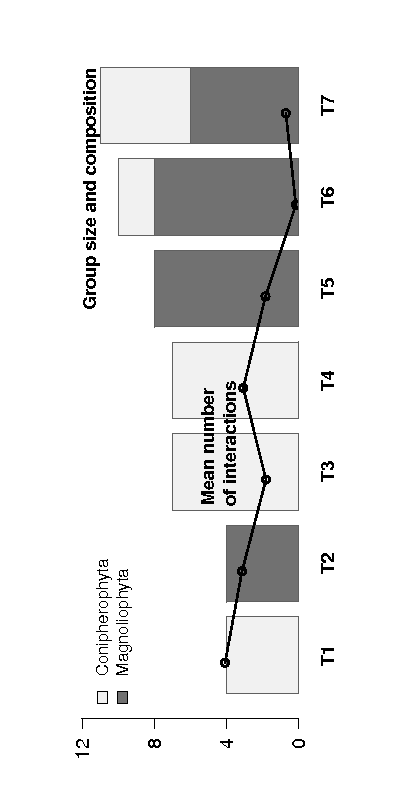
\includegraphics[width=.5\textheight, height=.6\textwidth, angle=270]{\fignet/MRV10_AoAS_Q7_group}
        }
    \end{tabular}
  \end{tabular}
  }

%====================================================================
\frame{ \frametitle{Accounting for the taxonomic distance $d_{ij}$}
  \begin{tabular}{cc}
%     \hspace{-.05\textwidth}
    \begin{tabular}{p{.4\textwidth}}
      \paragraph{Model:} \refer{MRV10}
      $$
      Y_{ij} \sim \Pcal[\lambda_{k\ell} \; \emphase{e^{\beta d_{ij}}}].
      $$

      \bigskip \pause
      \paragraph{Results:} $\widehat{\beta} = -0.317$. \\
%       \ra for $\overline{d} = 3.82$, 
%       $$
%       e^{\widehat{\beta}\overline{d}} = .298
%       $$
%       \ra The mean number of shared parasites \emphase{decreases as the distance increases}.
      
      \bigskip \bigskip 
      \paragraph{Pseudo-BIC:} $K=4$ groups.
    \end{tabular}
    & 
    \begin{tabular}{c}
      {\tiny
        \begin{tabular}{c|cccc}
          $\widehat{\lambda}_{k\ell}$ & T'1 & T'2 & T'3 & T'4 \\ 
          \hline \hline
          T'1 & 0.75 & 2.46 & 0.40 & 3.77 \\
          T'2 &  & 4.30 & 0.52 & 8.77 \\ 
          T'3 &  &  & 0.080 & 1.05 \\ 
          T'4 &  &  &  & 14.22 \\
          \hline \hline
          $\widehat{\pi}_k$ & 17.7 & 21.5 & 23.5 & 37.3 \\
          \hline \hline
          $\widehat{\beta}$ & \multicolumn{4}{c}{-0.317}
        \end{tabular}
        } \\ 
      \pause
      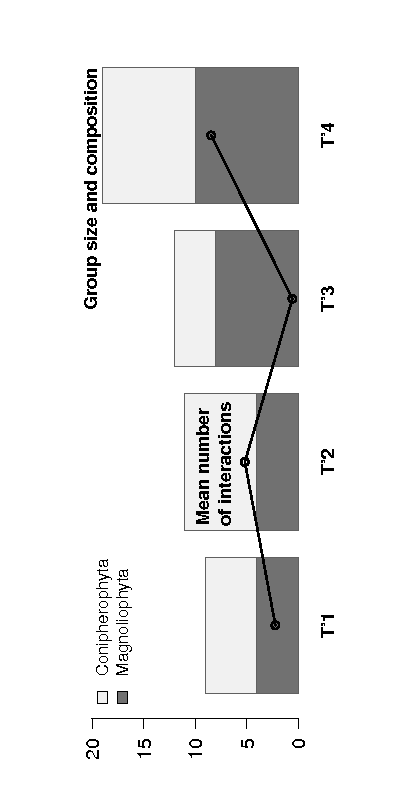
\includegraphics[width=.5\textheight, height=.5\textwidth, angle=270]{\fignet/MRV10_AoAS_Q4_group}
    \end{tabular}
  \end{tabular}
  
%   \ra Groups are no longer associated with the phylogenetic
%   structure. \\
%   \ra Mixture $=$ \emphase{residual heterogeneity} of the regression.
  }

%====================================================================
\frame{ \frametitle{Problem}

  \paragraph{Ecological network} $Y = (Y_{ij})_{1 \leq i, j \leq n}$: interactions between $n$ tree species:
  $$
  Y_{ij} = \Ibb\{i \sim j\}  = \Ibb\{\text{$i$ and $j$ share some fungal parasite}\}
  $$
  \ra in this talk, \emphase{binary networks only}.
  
  \bigskip \bigskip \pause
  \paragraph{+ Edge covariates} $x = (x_{ij})_{1 \leq i, j \leq n}$:
  \begin{itemize}
   \item $x^1_{ij}$ = phylogenetic distance between $i$ and $j$,
   \item $x^2_{ij}$ = geographic distance between the typical habitat of $i$ and $j$,
   \item ...
  \end{itemize}

  \bigskip \bigskip \pause
  \begin{overprint}
   \onslide<3>
  \paragraph{Questions:} 
  \begin{itemize}
   \item Can we explain the topology of $Y$ based on $x$? 
   \item Is there a residual heterogeneity in the network $Y$? 
  \end{itemize}
   \onslide<4>
  \paragraph{Questions:} 
  \begin{itemize}
   \item Can we explain the topology of $Y$ based on $x$? \qquad \ \ \emphase{\ra logistic regression}
   \item Is there a residual heterogeneity in the network $Y$? \quad \emphase{\ra $W$-graph}
  \end{itemize}
  \end{overprint}
  }
  
%====================================================================
\frame{\frametitle{Outline} \tableofcontents}

% %====================================================================
% %====================================================================
% \section{Variational Bayes inference}
% \frame{\frametitle{Outline} \tableofcontents[currentsection]}

%====================================================================
%====================================================================
\section{Reminder of variational Bayes inference}
\frame{\frametitle{Outline} \tableofcontents[currentsection]}
%====================================================================
\frame{\frametitle{Variational Bayes inference: General principle}

  \bigskip
  $Y=$ observed data, $Z=$ latent variable, $\theta=$ parameter. 
  
  \bigskip
  Frequentist or Bayesian inference requires
  $$
  p(Z|Y), \qquad p(\theta|Y), \qquad p(\theta, Z|Y).
  $$
  
  \pause \bigskip \bigskip
  \paragraph{Variational inference:}
%   $$
%   \fbox{\text{\paragraph{Variational inference:} find } \pt(\cdot) \approx p(\cdot|Y).}
%   $$
%   \paragraph{Variational inference:}
  $$
  \fbox{find \quad $\pt(\cdot) \approx p(\cdot|Y)$}
  $$

  
  \pause \bigskip \bigskip 
  Typically \refer{Jaa00,Min05,WaJ08}
  $$
  \pt = \arg\min_{q \in \Qcal} D[q(\cdot) \ \| \ p(\cdot|Y)]
  $$
  \begin{tabular}{cc}
   \begin{tabular}{p{.45\textwidth}}
   \vspace{-.05\textheight}
    \begin{itemize}
    \item $D[q\ \| \ p] = KL[q\ \| \ p]$; 
    \item $\pt(\theta) = \Ncal$;
    \end{itemize}
   \end{tabular}
   &
   \begin{tabular}{p{.45\textwidth}}
   \vspace{-.05\textheight}
    \begin{itemize}
    \item $\pt(Z) = \prod_i q_i(Z_i)$;
    \item $\pt(\theta, Z) = \pt(\theta) \pt(Z)$.
    \end{itemize}
   \end{tabular}
  \end{tabular}

}

%====================================================================
\frame{\frametitle{Variational Bayes inference: Some tools}

  \bigskip
  \paragraph{Latent variable models:} mean field approximation 
  $$
  \pt(\theta, Z) := \pt(\theta) \emphase{\times} \pt(Z),
  $$
  The VBEM algorithm \refer{BeG03} achieves
  $$
  \min_{\pt} \; KL[\pt(\theta, Z) \ \| \ p(\theta, Z|Y)] 
  \quad \Leftrightarrow \quad
  \max_{\pt} \; \log p(Y) - KL[\pt(\theta, Z) \ \| \ p(\theta, Z|Y)] 
  $$
%   \ra Close-form update formulas in the conjugate prior-exponential family setting. \\
%   \ra Computable lower bound of $p(Y)$ 

  \bigskip \bigskip \pause
  \paragraph{Bayesian model averaging (BMA) \refer{HMR99}:} Consider models $M_1, \dots, M_K, \dots$ 
  $$
  \Esp[h(\theta) | Y] = \sum_{K} \emphase{p(K|Y)} ~ \Esp[h(\theta) | Y, K]
  $$
  \pause
  Variational approximation of $p(K|Y)$ \refer{VMR12}:
  $$
  \pt(K) 
  \quad \propto \quad p(K|Y)~ e^{-\emphase{KL_K^*}}
  \quad \propto \quad p(K) ~ e^{\emphase{\log p(Y|K) - KL_K^*}} 
  $$ 
  where $KL_K^* =$ minimized $KL$ divergence for model $M_K$. 
%   
%   \bigskip \bigskip \pause
%   \paragraph{Variational BMA:} $\Espt[h(\theta)] = \sum_K \emphase{\pt(K)} ~ \Espt[h(\theta)].$

}


%====================================================================
%====================================================================
\section{Logistic regression}
\frame{\frametitle{Outline} \tableofcontents[currentsection]}
%====================================================================
\frame{\frametitle{Logistic regression}

  \paragraph{Forget about the network structure:} $(Y_{ij})$ are independent
  $$
  Y_{ij} \sim \Bcal[g(x_{ij}^\intercal \beta)], 
  \qquad
  g(u) = 1 / (1 + e^{-u})
  $$
  
  \bigskip \bigskip \pause
  \paragraph{Bayesian inference.} Prior on $\beta$:
  $$
  \beta \sim \Ncal(m, G^{-1})
  $$
  
  \bigskip
  {Posterior distribution:} 
  $$
  p(\beta|Y) \propto p(\beta) p(Y|\beta)
  $$
  \begin{itemize}
   \item No nice conjugacy holds for the normal prior / logistic regression model.
   \item No close form for the posterior $p(\beta | Y)$.
  \end{itemize}

  }
  
%====================================================================
\frame{\frametitle{Variational Bayes inference}

  \begin{tabular}{ll}
    \hspace{-.05\textwidth}
    \begin{tabular}{p{.5\textwidth}}
    Nasty term in $\log p(Y | \beta)$:
    $$
    -\log (1 + e^{-x_{ij} \beta}).
    $$
    
    \pause \bigskip
    \refer{JaJ00}: quadratic lower bound of $\log p(\beta, Y)$ to get 
    $$
    p(\beta|Y) \approx \pt(\beta) = \Ncal(\beta; \widetilde{m}, \widetilde{G}^{-1}).
    $$
    \end{tabular}
    & 
    \hspace{-.05\textwidth}
    \begin{tabular}{p{.5\textwidth}}
      \includegraphics[width=.45\textwidth]{../FIGURES/ApproxJaJ00}
    \end{tabular}
  \end{tabular}

%   
%   \pause \bigskip
%   \refer{JaJ00} observe that 
%   $$
%   -\log (1 + e^{-u}) = \frac{u}2 - \log(e^{u/2} + e^{-u/2})
%   $$ 
%   where $- \log(e^{u/2} + e^{-u/2})$ is convex in $u^2$, so a quadratic lower bounding of $\log p(\beta, Y)$ can be derived to get 
%   $$
%   p(\beta|Y) \approx \pt(\beta) = \Ncal(\beta; \mu_\beta, S_\beta).
%   $$
  
  \pause
  \paragraph{Example: Tree network.} $n = 51$ tree species, ($N = 1275$ pairs), 3 distances:
  $$
  \begin{array}{rrrrr}
   & \text{intercept} & \text{genetic} & \text{geographic} & \text{taxonomic} \\
   \hline
   \mu_{\beta} & 0.221 & 0.060 & -0.337 & -0.811 \\
   \sigma_{\beta} & 0.058 & 0.062 & 0.059 & 0.060 \\
  \end{array}
  $$

}

%====================================================================
%====================================================================
\section{$W$-graphs and graphon}
\frame{\frametitle{Outline} \tableofcontents[currentsection]}
%====================================================================
\frame{\frametitle{Latent space models}

%   Most observed networks are heterogeneous in terms of degree distribution, node centrality, existence of clusters, ...
  
  \bigskip 
  \paragraph{Generic framework \refer{BJR07}:}
  \begin{itemize}
   \item Latent variable for node $i$: $Z_i \sim \pi$.
   \item Edges $Y_{ij}$ conditionally independent: 
  \end{itemize}
  $$
  (Z_i) \text{ iid } \sim \pi, 
  \qquad 
  Y_{ij} \ | \ (Z_i): Y_{ij} \sim \Bcal[\emphase{\gamma(Z_i, Z_j)}]
  $$ 
  
  \bigskip \pause
  Includes 
%   \Refer{Matias and R. (2014)}\nocite{MaR14}: 
  \refer{MaR14}: 
  \begin{itemize}
   \item stochastic block-model \refer{FrH82}, 
   \item latent position models \refer{HRH02,HRT07,DPV10}, 
   \item $W$-graph \refer{LoS06,DiJ08}
   $$
   \text{\ra \emphase{'limit' model of most of these models}.}
   $$
  \end{itemize}
  
  \bigskip \pause
  \paragraph{Intricate dependency structure:} sampling and/or approximation is required for the inference of $p(Z, \theta|Y)$
  }

%====================================================================
\frame{ \frametitle{$W$-graph (graphon)  model}

  \begin{tabular}{cc}
    \hspace{-.02\textwidth}
    \begin{tabular}{p{.5\textwidth}}
	 Latent variables:
	 $$
	 (U_i) \text{ iid } \sim \Ucal_{[0, 1]},
	 $$ ~\\
	 \emphase{Graphon} function $\gamma$:
	 $$
	 \gamma(u, v): [0, 1]^2 \mapsto [0, 1]
	 $$ ~\\    
	 Edges:
	 $$
	 P(Y_{ij} = 1|U_i, U_j) = \gamma(U_i, U_j)
	 $$    
	 \end{tabular}
    & 
    \hspace{-.1\textwidth}
    \begin{tabular}{p{.5\textwidth}}
	 Graphon function $\gamma(u, v)$ \\
      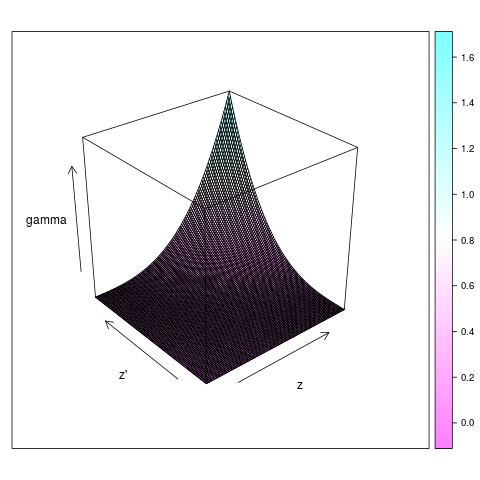
\includegraphics[width=.5\textwidth]{../FIGURES/FigCLADAG-W-graphon} \\
    \end{tabular}
  \end{tabular}
  
 }

%====================================================================
\frame{\frametitle{Some typical graphon functions}

  Graphon function $\gamma$: a global picture of the network's topology.

  \bigskip \bigskip 
  \centerline{
  \begin{tabular}{ccc}
  'Scale free' & Community & Small world \\
  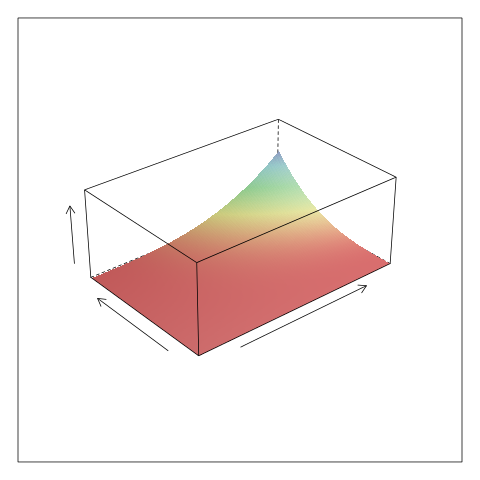
\includegraphics[width=.3\textwidth]{../FIGURES/EDD-ScaleFreeTrueGraphon} &
  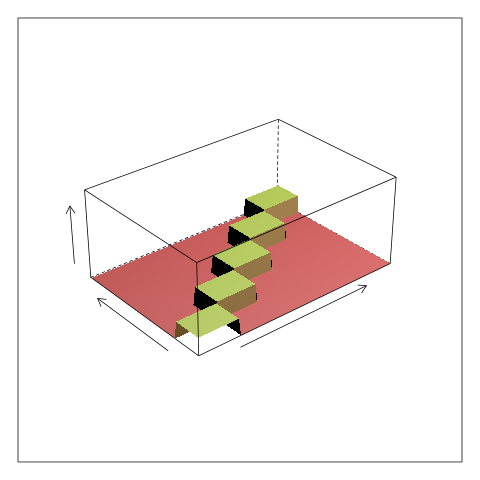
\includegraphics[width=.3\textwidth]{../FIGURES/CommunityTrueGraphon} &
  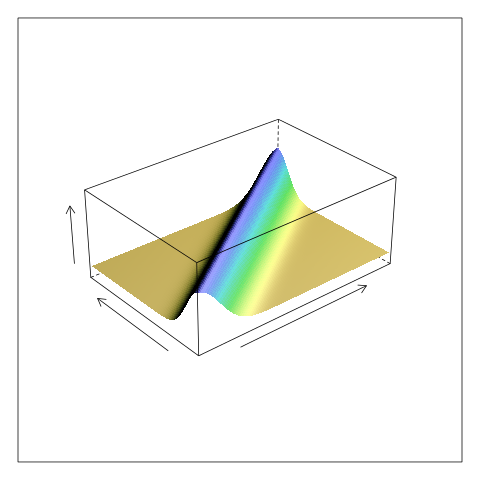
\includegraphics[width=.3\textwidth]{../FIGURES/SmallWorldTrueGraphon} 
  \end{tabular}
  } 
  
  \bigskip \pause
  \paragraph{Remark:} $\gamma(\cdot, \cdot) = $cst \ra ER model
  
}

%====================================================================
\frame{ \frametitle{Variational Bayes inference of the graphon (1/3)}

  \paragraph{Stochastic Block-model (SBM) is a $W$-graph model.} 

  \bigskip
  \begin{tabular}{cc}
    \hspace{-.02\textwidth}
    \begin{tabular}{p{.5\textwidth}}
        \vspace{-.5\textheight}
	 Latent variables:
	 $$
	 (Z_i) \text{ iid } \sim \Mcal(1, \pi)
	 $$
	 Blockwise constant graphon:
	 $$
	 \gamma(z, z') = \gamma_{k\ell}
	 $$
	 Edges:
	 \begin{eqnarray*}
	 P(Y_{ij} = 1|Z_i, Z_j) & = & \gamma(Z_i, Z_j) \\
% 	 \logit (~"~) & = & Z_i^\intercal \alpha Z_j \\
% 	 \alpha & = & \logit(\gamma)
	 \end{eqnarray*}    
	 \end{tabular}
    & 
    \hspace{-.1\textwidth} \pause
    \begin{tabular}{p{.5\textwidth}}
	 \begin{overprint}
	 \onslide<2>
	 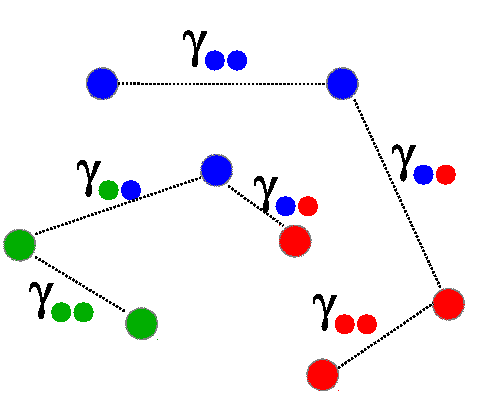
\includegraphics[width=.45\textwidth]{../FIGURES/FigSBM-Model-3-red} 
	 \onslide<3>
	 Graphon function of $SBM_K$ \\
	 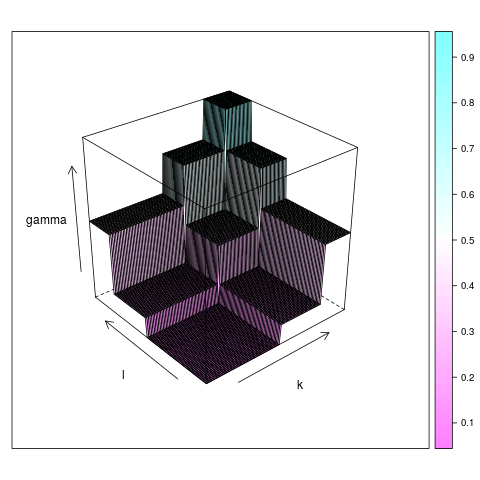
\includegraphics[width=.45\textwidth]{../FIGURES/FigCLADAG-SBM-graphon} 
	 \end{overprint}
    \end{tabular}
  \end{tabular} 

  \vspace{-.5\textheight}
  \onslide+<3>{\ra block widths $= \pi_k$, block heights $\gamma_{k\ell}$}
 }

%====================================================================
\frame{ \frametitle{Variational Bayes inference of the graphon (2/3)}

  \bigskip 
  \begin{tabular}{cc}
    \hspace{-.05\textwidth}
    \begin{tabular}{p{.45\textwidth}}
    \paragraph{VBEM for SBM:} conjugate prior-exponential family setting %\\
    \refer{LBA12}.
    
    \bigskip \bigskip \pause
    Approximate posteriors
    \begin{eqnarray*}
    \pt(\pi) & = & \Dcal(\widetilde{\pi}) \\
    \pt(\gamma_{k\ell}) & = & \Beta(\widetilde{\gamma}^0_{k\ell}, \widetilde{\gamma}^1_{k\ell}) \\
    \pt(Z_i) & = & \Mcal(1; \widetilde{\tau}_i) \\
    \end{eqnarray*} 
    \end{tabular}
    & 
    \hspace{-.05\textwidth} \pause
    \begin{tabular}{p{.5\textwidth}}
	 Posterior mean $\Espt^{SBM}_K[\gamma(u, v)]$ \\
      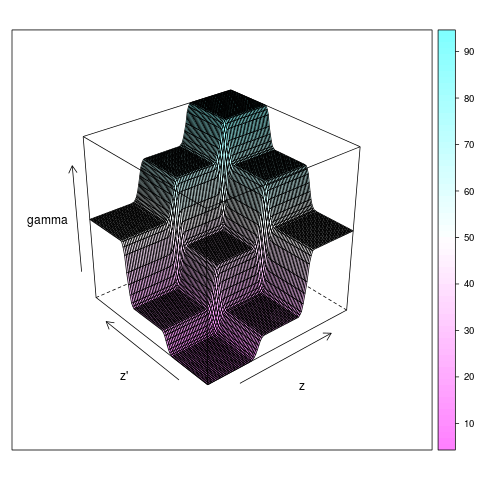
\includegraphics[width=.45\textwidth]{../FIGURES/FigGraphon-SBM-average} 
    \end{tabular}
  \end{tabular}
}

%====================================================================
\frame{ \frametitle{Variational Bayes inference of the graphon (3/3)}

  \paragraph{Variational Bayes model averaging.}
  \begin{itemize}
   \item Each auxiliary model $SBM_K$ provides an estimates of $\gamma$ as:
   $$
   \widehat{\gamma}_K(u, v) = \Espt_K^{SBM}[\gamma(u, v)].
   $$ \\~
   \item VB inference also provides an approximation of the posterior probability of each auxiliary model $SBM_K$:
   $$
   \pt(K) \approx p(K|Y)
   $$ \\~
   \item A averaged estimate of $\gamma$ is given by 
%    \Refer{Latouche and R. (2015)}\nocite{LaR15}:
   \refer{LaR15}:
   $$
   \Espt[\gamma(u, v)] = \sum_K \emphase{\pt(K)} ~ \Espt_K^{SBM}[\gamma(u,
   v)].
   $$
  \end{itemize}

}

%====================================================================
\frame{\frametitle{Example: Tree network}

  $n = 51$ tree species. Inferred graphon function:
  $$
  \includegraphics[height=.5\textheight]{../FIGURES/treed0} 
  $$
  }

%====================================================================
\frame{\frametitle{Example: Political blog network}

  $n = 196$ blogs. Inferred graphon function:
  $$
  \includegraphics[height=.5\textheight]{../FIGURES/blogd0} 
  $$
  
  \pause
  \begin{itemize}
   \item Graphical representation of the network.
   \item Interpretability...
  \end{itemize}
  }

%====================================================================
%====================================================================
\section{Goodness-of-fit}
\frame{\frametitle{Outline} \tableofcontents[currentsection]}
%====================================================================
\frame{\frametitle{Back to the original problem}

  \paragraph{Data:}
  \begin{itemize}
   \item $Y =$ observed (binary) network
   \item $x = $ covariates
  \end{itemize}

  \bigskip \bigskip 
  \paragraph{Questions:}
  \begin{itemize}
   \item Does $x$ explain the topology of $Y$?
   \item Residual (wrt $x$) heterogeneity in $Y$?
  \end{itemize}

}

%====================================================================
\frame{\frametitle{Combined model}

  \bigskip
  \paragraph{Logistic regression:}
  $$
  \logit~P(Y_{ij} = 1) = 
  \emphase{\beta_0} + \sum_k \beta_k x_{ij}^k
  $$

  \bigskip \bigskip \pause
  \paragraph{Logistic regression + graphon residual term:} $(U_i)$ iid $\sim \Ucal[0, 1]$,
  $$
  \logit~P(Y_{ij} = 1 |U_i, U_j) = 
  \emphase{\phi(U_i, U_j)} + \sum_k \beta_k x_{ij}^k
  $$

  \bigskip \bigskip \pause
  \paragraph{Goodness of fit \refer{LRO15}:} Check if
  $$
  \phi(u, v) = \cst \qquad (= \beta_0)
  $$
  }

%====================================================================
\frame{\frametitle{Goodness-of-fit as model comparison}

  \bigskip
  \paragraph{Auxiliary model $M_K$:} % $Z_i \sim \Mcal_K(1; \pi)$, $\alpha: K \times K$,
  $$
  \logit~P(Y_{ij} = 1 | U_i, U_j, K) = \emphase{\phi_K^{SBM}(U_i, U_j)} + \sum_k \beta_k x_{ij}^k.
  $$
%   \emphase{Model $M_K =$} logistic regression + $K$-class SBM residual. 
  
  \bigskip \bigskip \pause
  \paragraph{Goodness of fit:} 
  $$
  \begin{array}{rclcl}
   H_0 & = & \{\text{logistic regression is sufficient}\} & = & M_1 \\
   H_1 & = & \{\text{logistic regression is not sufficient}\} & = & \bigcup_{K > 1} M_K 
  \end{array}
  $$
  GOF is a assessed if
  $$
  p(H_0|Y) = p(M_1|Y) \text{ is large.}
  $$

%   \pause \bigskip \bigskip
%   \paragraph{Model averaging} yields
%   $$
%   p(\phi | Y) = \sum_k p(K|Y) \ p(\phi_K^{SBM} | Y)
%   $$

  }

%====================================================================
\frame{\frametitle{Variational Bayes inference}

  \bigskip
  \paragraph{VBEM:} A global variational Bayes EM algorithm can be designed to obtain all needed (approximate) posteriors:
  \begin{eqnarray*}
   p(\theta, Z, K|Y) & \approx & \pt(\theta, Z, K) 
   \quad = \quad \pt(K) \; \pt(\theta |K) \; \emphase{\times} \; \pt(Z | K) \\
   & = & \pt(K) \; \left(\pt(\alpha |K) \; \pt(\beta |K) \; \pt(\pi |K)\right) \; \emphase{\times} \; \left(\emphase{\prod_i} \; \pt(Z_i | K)\right)
  \end{eqnarray*}
%   $$
%   \pt(\beta|K), \qquad \pt(\pi|K), \qquad \pt(\alpha|K), \qquad \pt(Z|K), \qquad \pt(K).
%   $$
  
  \bigskip \pause
  \paragraph{Posterior quantities of interest:}
  \begin{itemize}
   \item Goodness of fit criterion:
   $$
   p(H_0|Y) \approx \Pt(K=1)
   $$
   \item Residual graphon:
   $$
   \widehat{\phi}(u, v) = \sum_K \pt(K) ~ \Espt[\phi^{SBM}_K(u, v)]
   $$
  \end{itemize}
  }

%====================================================================
%====================================================================
\section{Illustrations}
\frame{\frametitle{Outline} \tableofcontents[currentsection]}
%====================================================================
\frame{\frametitle{Some examples}

\begin{centering}
\begin{tabular}{l|cccc}
 network & size ($n$) & nb. covariates ($d$) & density &$\hat{p}(H_0|Y)$ \\ 
  \hline
Blog & 196 & 3 &0.075&  3e-172 \\
Tree & 51 & 3 & 0.54 & 2e-115\\
Karate & 34 & 8 &0.14 & 3e-2 \\
Florentine (marriage) & 16 & 3 & 0.17 & 0.995 \\
Florentine (business) & 16 & 3 & 0.125 & 0.991 \\
Faux Dixon High & 248 & 17 & 0.02 & 1 \\
CKM & 219 & 39 & 0.015 & 1 \\
AddHealth 67 & 530 & 21 & 0.007& 2e-25 \\
\end{tabular}
\end{centering}
}

%====================================================================
\frame{\frametitle{Political blog network}

  $n = 196$ blogs ($N = 19110$ pairs), 3 covariates, density $= .075$ 

  \bigskip
  \begin{tabular}{cc}
    \begin{tabular}{p{.5\textwidth}}
	 Inferred graphon (no covariate) \\ ~\\
	 \includegraphics[height=.4\textheight]{../FIGURES/blogd0} \\ ~\\
	 ~
    \end{tabular}
    & 
    \hspace{-.05\textwidth}
    \begin{tabular}{p{.5\textwidth}}
	 Residual graphon (3 covariates) \\ ~\\
	 \includegraphics[height=.4\textheight]{../FIGURES/blogd3} \\ ~\\
	 $\Pt(H_0) \simeq 10^{-172}$
    \end{tabular}
  \end{tabular}
  }

%====================================================================
\frame{\frametitle{Tree network}

  $n = 51$ species ($N = 1275$ pairs), 3 covariates, density $= .54$ 

  \bigskip
  \begin{tabular}{cc}
    \begin{tabular}{p{.5\textwidth}}
	 Inferred graphon (no covariate) \\ ~\\
	 \includegraphics[height=.4\textheight]{../FIGURES/treed0} \\ ~\\
	 ~
    \end{tabular}
    & 
    \hspace{-.05\textwidth}
    \begin{tabular}{p{.5\textwidth}}
	 Residual graphon (3 covariates) \\ ~\\
	 \includegraphics[height=.4\textheight]{../FIGURES/treed3} \\ ~\\
	 $\Pt(H_0) \simeq 10^{-115}$
    \end{tabular}
  \end{tabular}
  }

%====================================================================
\frame{\frametitle{Florentine business}

  $n = 16$ families ($N = 120$ pairs), 3 covariates, density $= .12$ 

  \bigskip
  \begin{tabular}{cc}
    \begin{tabular}{p{.5\textwidth}}
	 Inferred graphon (no covariate) \\ ~\\
	 \includegraphics[height=.4\textheight]{../FIGURES/businessd0} \\ ~\\
	 ~
    \end{tabular}
    & 
    \hspace{-.05\textwidth}
    \begin{tabular}{p{.5\textwidth}}
	 Residual graphon (3 covariates) \\ ~\\
	 \includegraphics[height=.4\textheight]{../FIGURES/businessd3} \\ ~\\
	 $\Pt(H_0) = .991$
    \end{tabular}
  \end{tabular}
  }

%====================================================================
\frame{\frametitle{Physicians' friendship network}

  $n = 219$ individuals, 24 covariates (39 df), density $= .015$ 

  \bigskip
  \begin{tabular}{cc}
    \begin{tabular}{p{.5\textwidth}}
	 Inferred graphon (no covariate) \\ 
	 \includegraphics[height=.4\textheight]{../FIGURES/ckmd0} \\ ~\\
	 ~
    \end{tabular}
    & 
    \hspace{-.05\textwidth}
    \begin{tabular}{p{.5\textwidth}}
	 Residual graphon (3 covariates) \\ 
	 \includegraphics[height=.4\textheight]{../FIGURES/ckmd39} \\ 
	 $\Pt(H_0) \simeq 1$
    \end{tabular}
  \end{tabular}
  }

  

%====================================================================
%====================================================================
\section*{Discussion}
% \frame{\frametitle{Outline} \tableofcontents[currentsection]}
%====================================================================
\frame{\frametitle{Discussion}

  \paragraph{Contribution:}
  \begin{itemize}
   \item Generic logistic regression model with a network-oriented residual term.
   \item Detour through SBM provides a natural goodness-of-fit criterion.
   \item R package on \textcolor{blue}{\url{github.com/platouche/gofNetwork}} (soon on CRAN)
  \end{itemize}

  \bigskip \bigskip \pause
  \paragraph{Comments:}
  \begin{itemize}
   \item Strongly relies on variational Bayes approximation of the posteriors. 
   \item VBEM asymptotically accurate for logistic regression and SBM separately.
   \item No clue about accuracy in the combined model.
   \end{itemize}

  \bigskip \bigskip \pause
  \paragraph{On-going work:}
  \begin{itemize}
   \item Relevant {\sl edge} covariates made of {\sl node} covariates \refer{HGH08}.
   \item Efficient sampling in the true posterior using sequential importance sampling: \\ 
   \ra Move from $\pt(\cdot)$ to $p(\cdot|Y)$ using a tempering scheme.
   \end{itemize}
}

%====================================================================
%====================================================================
\backupbegin
\frame[allowframebreaks]{ \frametitle{References}
{\tiny
  \bibliography{/home/robin/Biblio/BibGene}
%   \bibliographystyle{astats}
  \bibliographystyle{plain}
  }
}

%====================================================================
%====================================================================
\appendix

\section*{Appendix}
%====================================================================
\frame{ \frametitle{Variational Bayes for heterogeneous network models}

  \begin{tabular}{cc}
    \hspace{-.05\textwidth}
    \begin{tabular}{p{.5\textwidth}}
      \onslide+<1->{
        \paragraph{Graphical model} formalism %\\
        \refer{Lau96}. \\ ~\\ }
        \onslide+<2->{\paragraph{'Frequentist' setting ($p(\cdot|\theta)$):}}
        \begin{itemize}
        \onslide+<2->{\item iid $Z_i$'s,}
        \onslide+<3->{\item $p(Y_{ij} | Z_i, Z_j)$,}
        \onslide+<4->{\item $p(Z_i, Z_j|Y)$: graph moralization,}
        \onslide+<5->{\item this holds for each pair $(i, j)$,}
        \end{itemize}
    \end{tabular}
    & 
    \hspace{-.02\textwidth}
    \begin{tabular}{p{.5\textwidth}}
	 \begin{overprint}
        \onslide<2>
        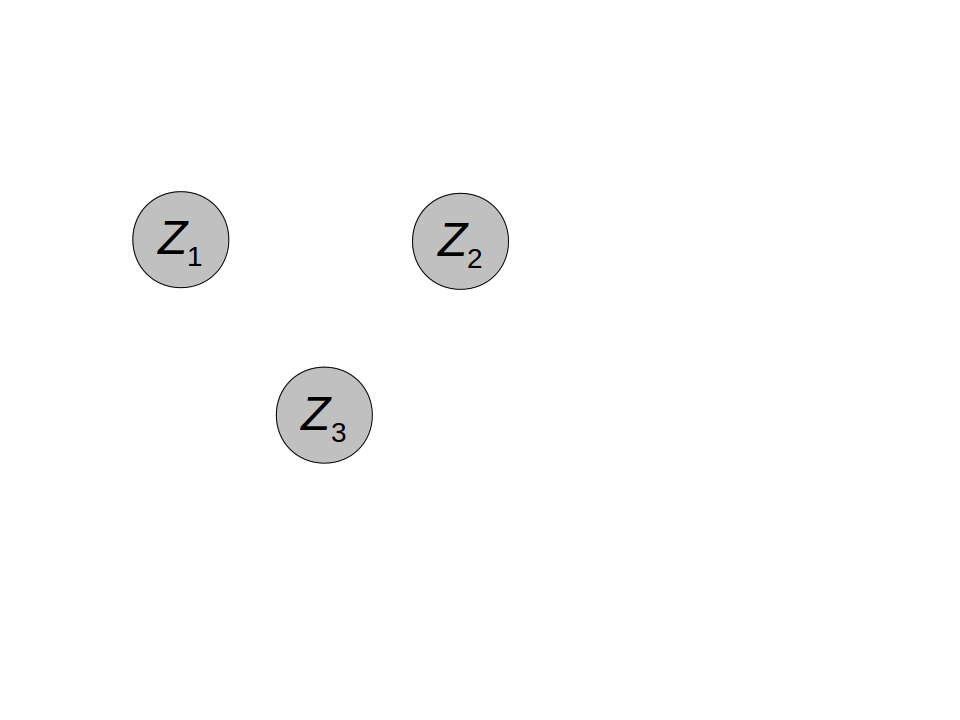
\includegraphics[width=0.6\textwidth]{../FIGURES/FigSBM-Z}
        \onslide<3>
        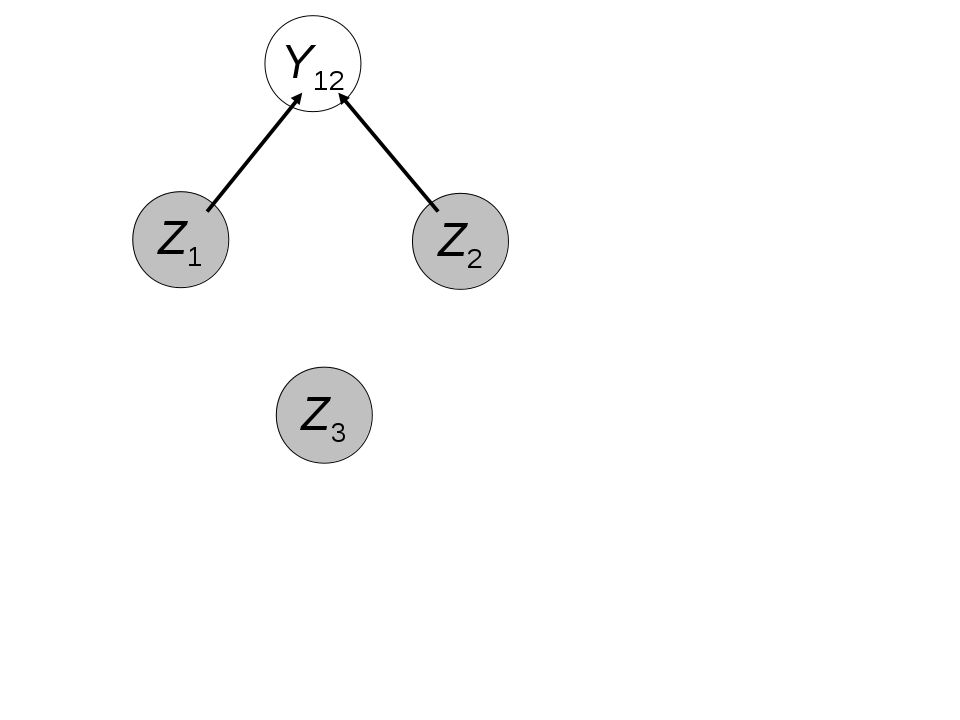
\includegraphics[width=0.6\textwidth]{../FIGURES/FigSBM-Z-Y12}
        \onslide<4>
        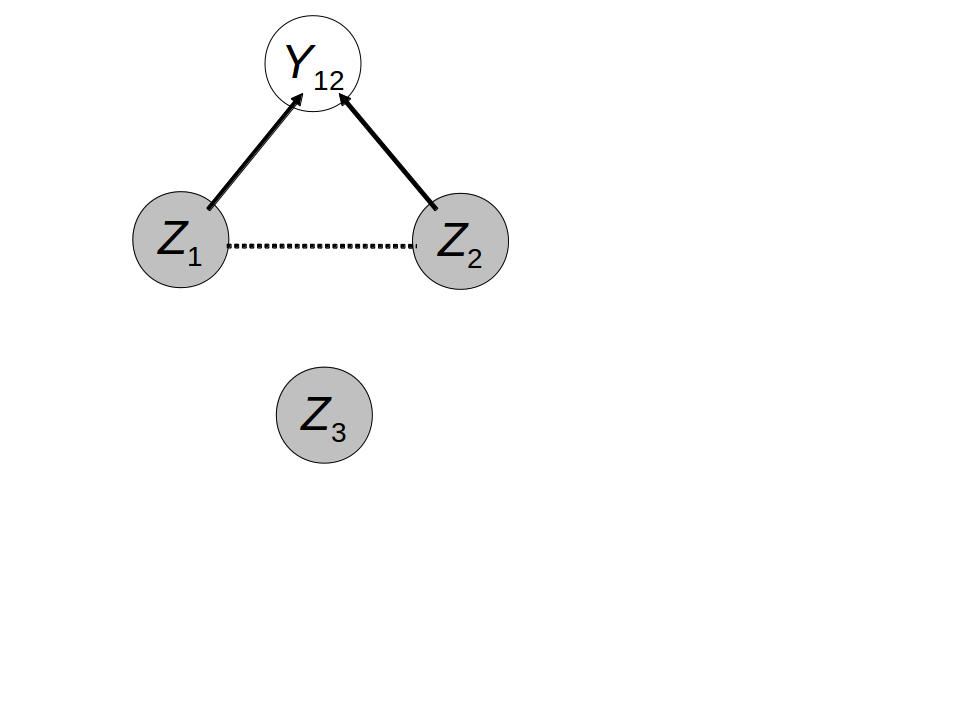
\includegraphics[width=0.6\textwidth]{../FIGURES/FigSBM-Z-Y12-Moral} 
        \onslide<5>
        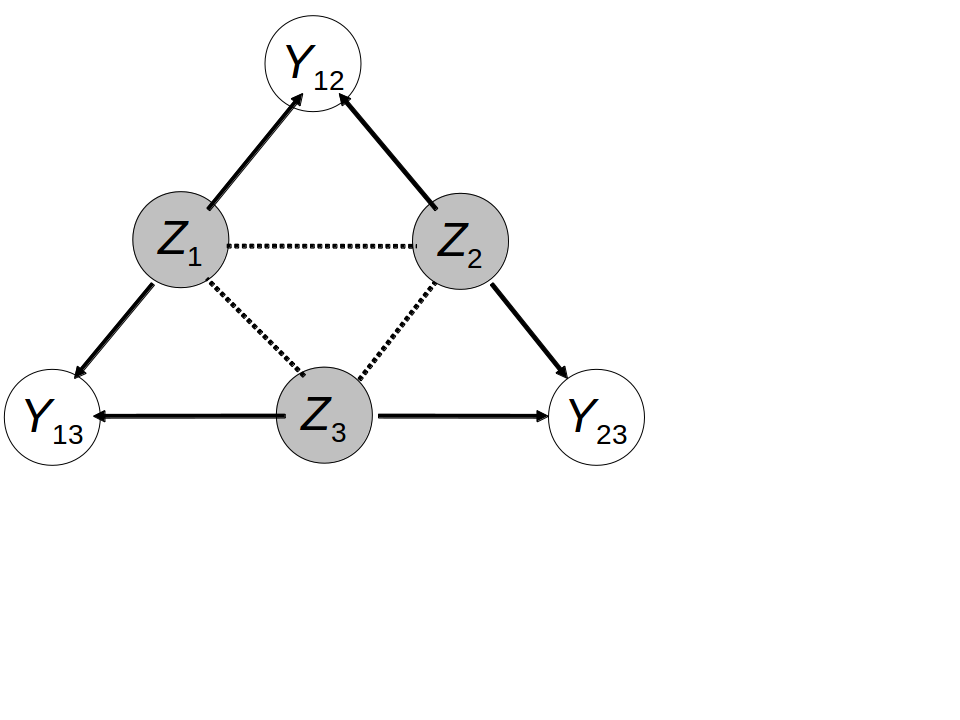
\includegraphics[width=0.6\textwidth]{../FIGURES/FigSBM-Z-Y-Moral} 
        \onslide<6>
        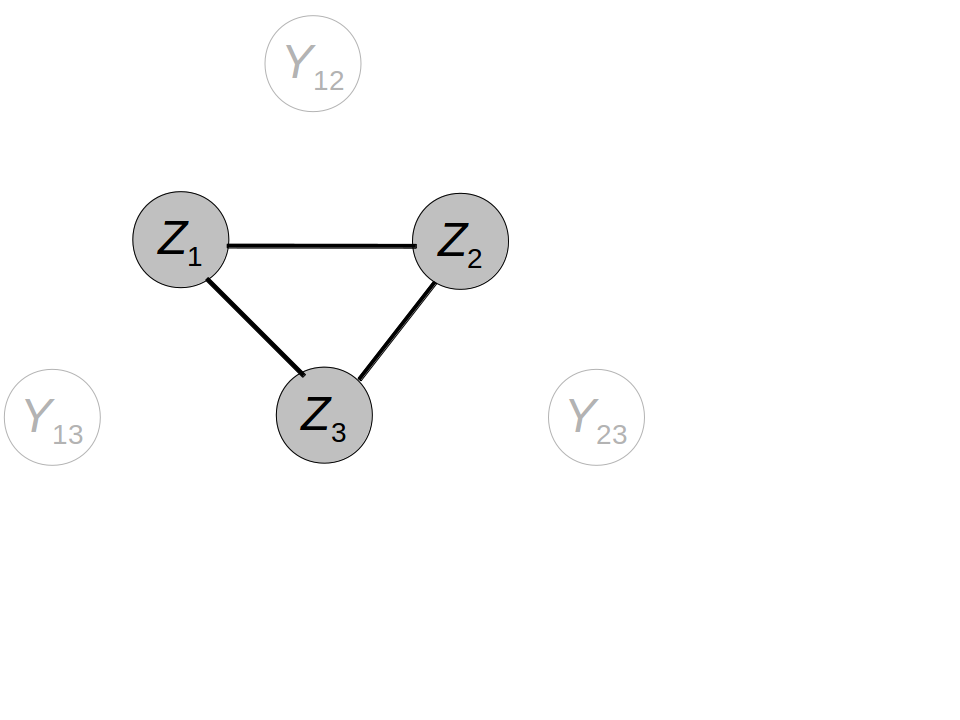
\includegraphics[width=0.6\textwidth]{../FIGURES/FigSBM-ZcondY}
        \onslide<7->
        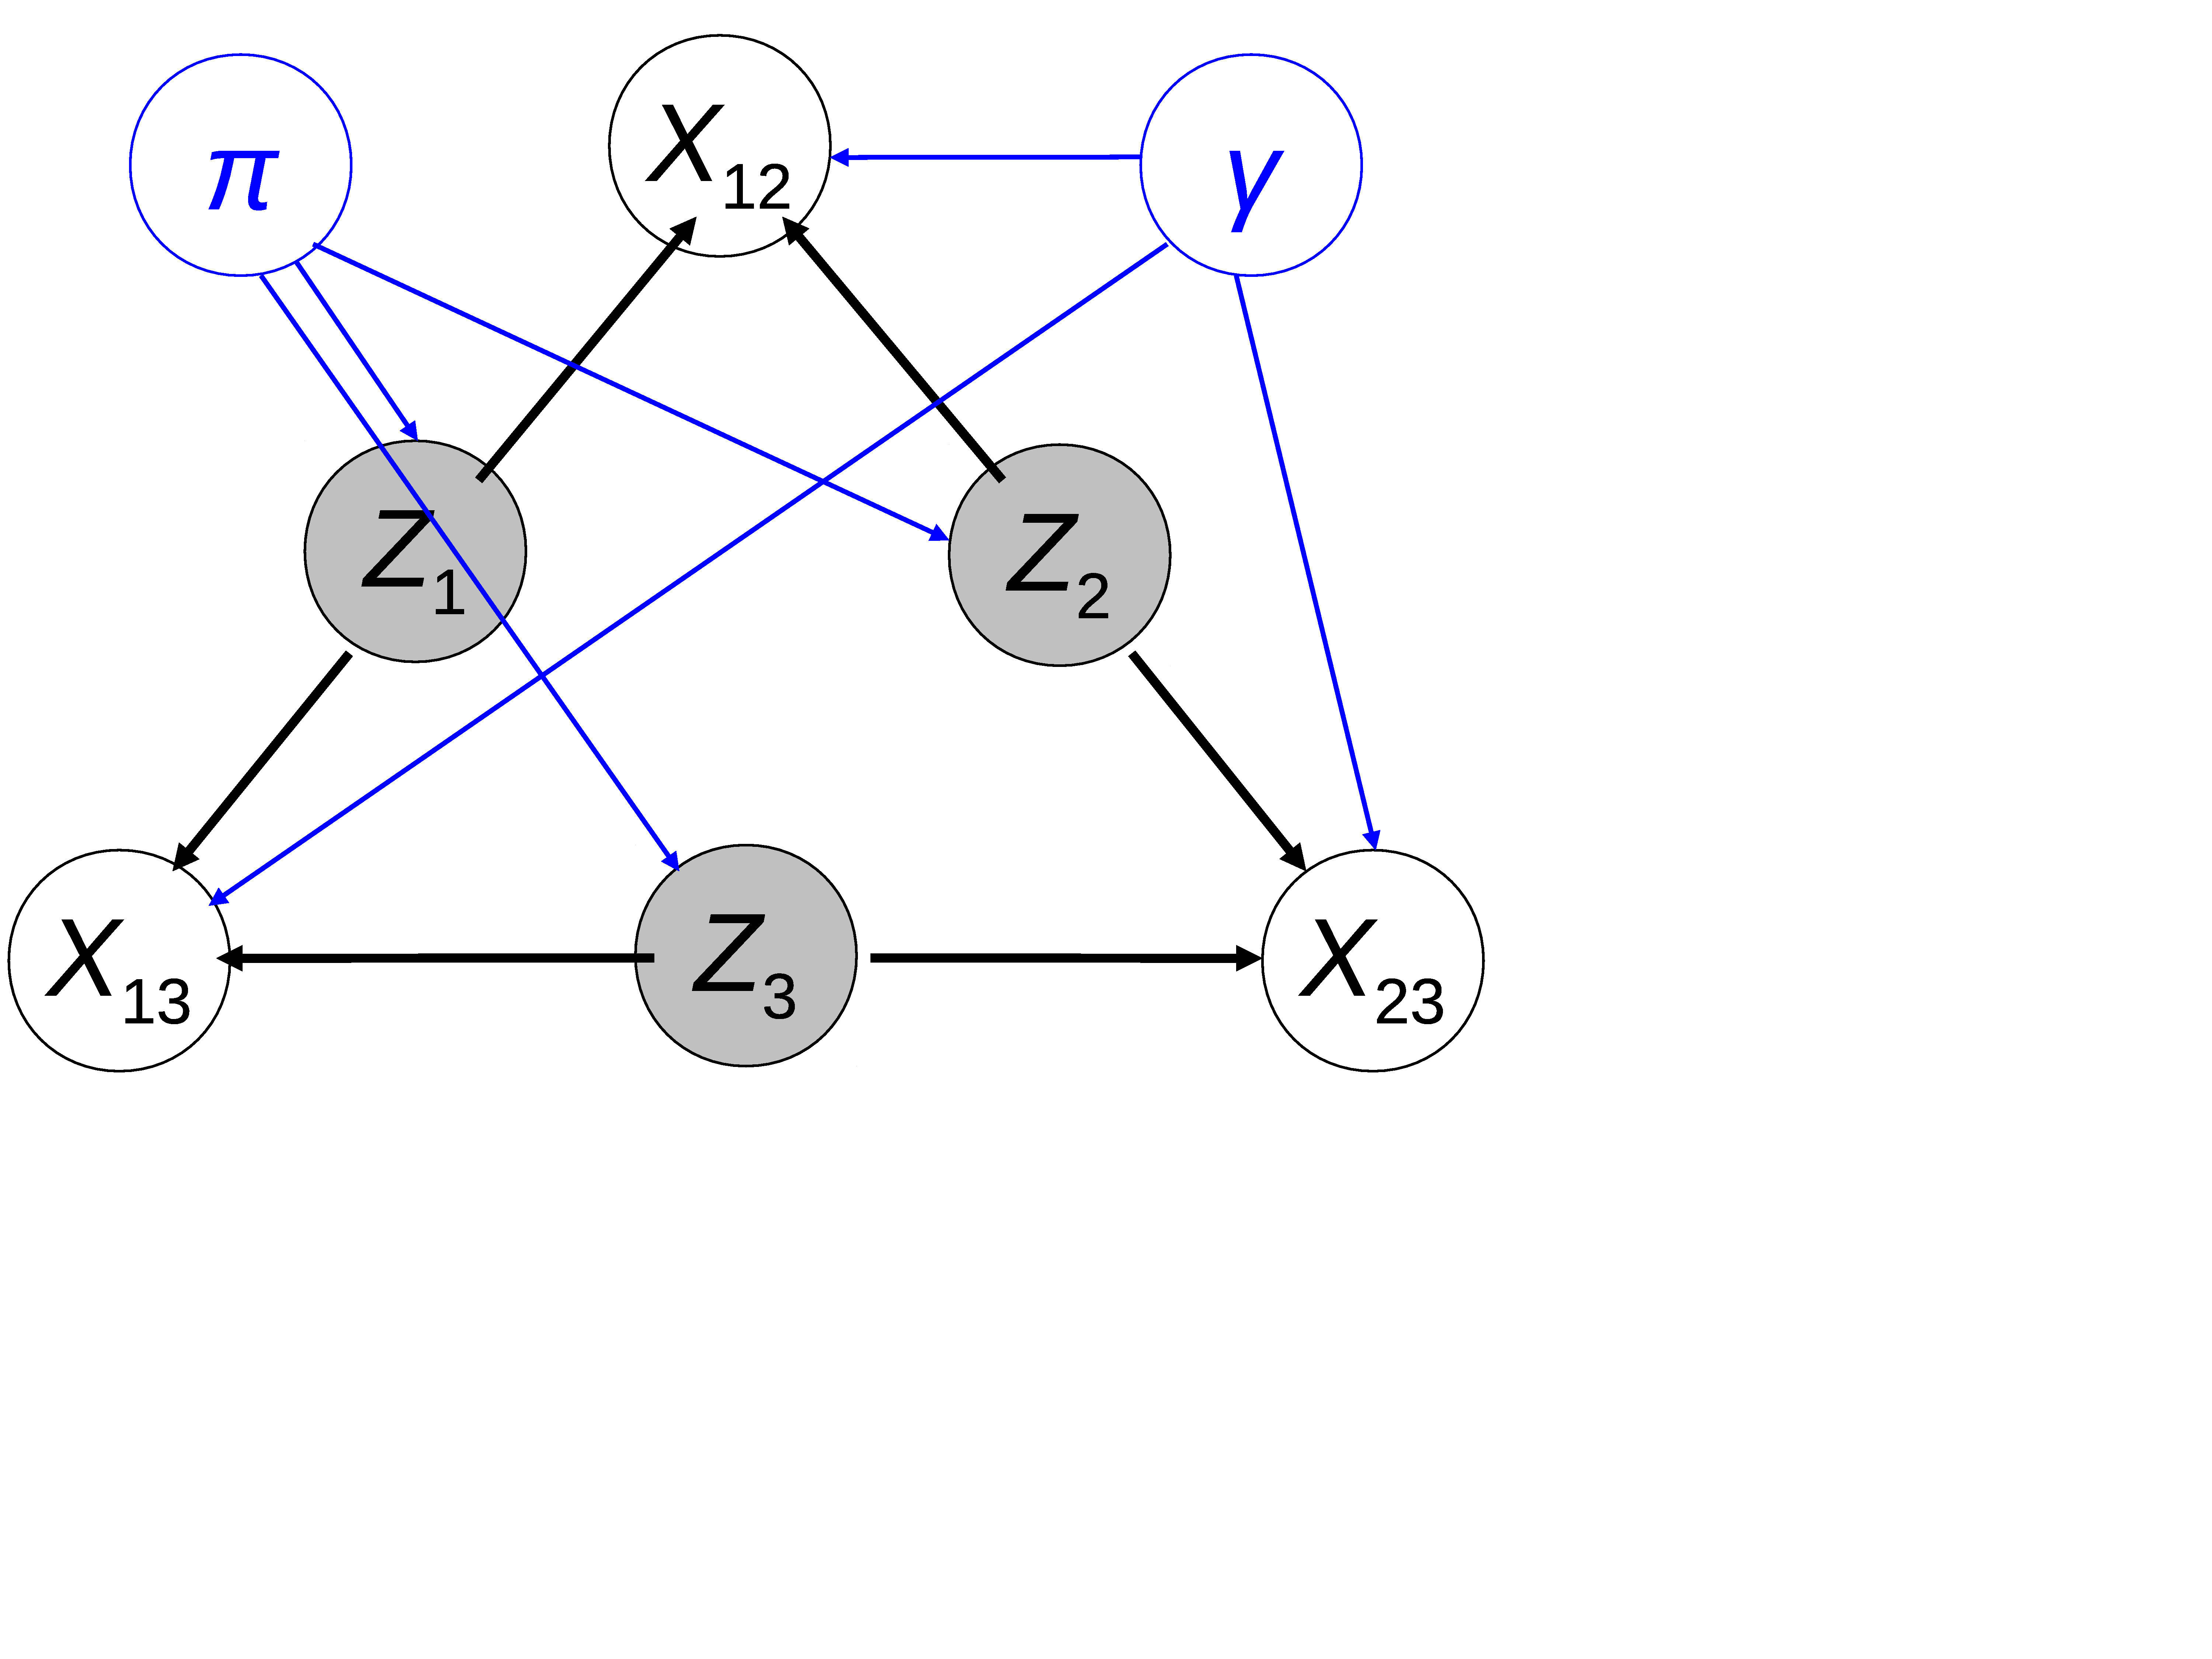
\includegraphics[width=0.6\textwidth]{../FIGURES/FigSBM-Bayes}
      \end{overprint}
    \end{tabular}
  \end{tabular}

  \vspace{-.05\textheight}
  \onslide<6->{
  \paragraph{Dependency graph of $p(Z|Y, \theta) =$ clique.}  \\
  \ra No factorization can be hoped (unlike for HMM). \\
  \ra $p(Z | Y, \theta)$ can not be computed (efficiently). \\ }
  \onslide<7>{
  \paragraph{Bayesian setting.} Things get worst.}

}

%====================================================================
\frame{ \frametitle{Accuracy of {\VBEM} estimates for SBM: Simulation study}

  \paragraph{Credibility intervals:}   $\pi_1$: $+$,
  $\gamma_{11}$: \textcolor{red}{$\triangle$}, $\gamma_{12}$:
  \textcolor{blue}{$\circ$}, $\gamma_{22}$: \textcolor{green}{$\bullet$} 
  $$
  \includegraphics[width=1\textwidth]{../FIGURES/im-ICQ2-2-new} 
  $$
  \pause
  \emphase{Width of the posterior credibility intervals.}
  {$\pi_1$}, \textcolor{red}{$\gamma_{11}$},
  \textcolor{blue}{$\gamma_{12}$}, \textcolor{green}{$\gamma_{22}$}
  \\
  \includegraphics[width=1\textwidth]{../FIGURES/im-ICQ2-3} \\
   \refer{GDR11}

 }
 
%====================================================================
\frame{\frametitle{A first criterion for goodness-of-fit: Motifs frequency}

  \vspace{-0.1\textheight}
  $$
  \begin{tabular}{cccccc}
  
\includegraphics[width=.1\textwidth]{../FIGURES/FigMotif-V}
  & 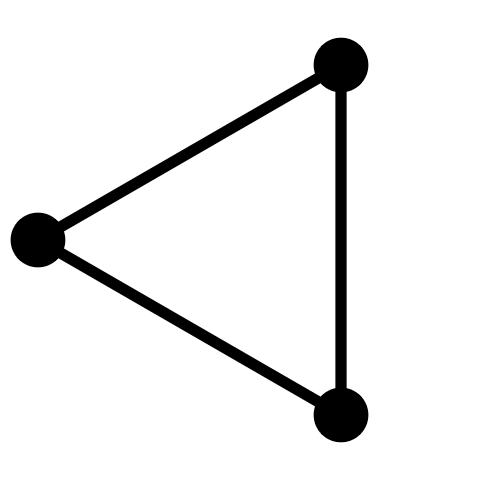
\includegraphics[width=.1\textwidth]{../FIGURES/FigMotif-Triangle}
  & 
\includegraphics[width=.1\textwidth]{../FIGURES/FigMotif-Square}
  & 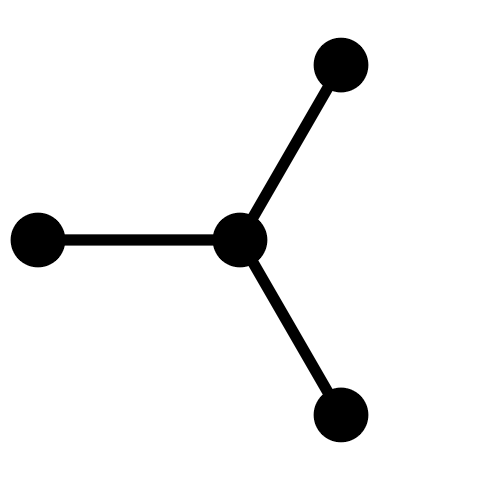
\includegraphics[width=.1\textwidth]{../FIGURES/FigMotif-Star3}
  & 
\includegraphics[width=.1\textwidth]{../FIGURES/FigMotif-Whisker}
  & 
\includegraphics[width=.1\textwidth]{../FIGURES/FigMotif-Clique4}
  \end{tabular}
  $$
  
  \begin{itemize}
  \item Network motifs have a biological or sociological interpretation in terms of building blocks of the global network 
  $$
  \text{\ra Triangles = 'friends of my friends are my friends'. }
  $$
  \item Latent space graph models only describe binary interactions, conditional on the latent positions
  \end{itemize} 
  
  \bigskip
  \ra Goodness of fit criterion based on motif frequencies? 
%   \Refer{Latouche and R. (2015)}\nocite{LaR15}.
  \refer{LaR15}.
    
}

%====================================================================
\frame{\frametitle{Moments of motif counts}

  \paragraph{First moments $\Esp N(m)$, $\Var N (m)$} known for exchangeable graphs (incl. SBM) \refer{PDK08}: 
  $$
  \Esp_{SBM} N(m) \propto  \mu_{SBM}(m), 
  \qquad 
  % =: f(\theta_{SBM}) %, \Var_{SBM(K)} N(m)
  \mu_{SBM}(m) = \text{motif occurrence probability.}
  $$
  $\Var N (m)$ depends on the frequency of super-motifs:
  $$
  \begin{tabular}{c|cc|ccc}
  Motif & \multicolumn{2}{c|}{1-node overlap} & \multicolumn{3}{c}{2-node overlap} \\
  \hline
  \begin{tikzpicture}
\node[node] (i) at (0*\edgeunit, 0*\edgeunit) {$\bullet$};
\node[node] (j) at (-0.435*\edgeunit, .87*\edgeunit) {$\bullet$};
\node[node] (k) at (.435*\edgeunit, .87*\edgeunit) {$\bullet$};
\draw[edge] (i) to (j); \draw[edge] (i) to (k);  
\end{tikzpicture}

  & \begin{tikzpicture}
\node[node] (i) at (-1*\edgeunit, 0*\edgeunit) {$\bullet$};
\node[node] (j) at (-.435*\edgeunit, .87*\edgeunit) {$\bullet$};
\node[node] (k) at (0*\edgeunit, 0*\edgeunit) {$\bullet$};
\node[node] (l) at (.435*\edgeunit, .87*\edgeunit) {$\bullet$};
\node[node] (m) at (\edgeunit, 0*\edgeunit) {$\bullet$};
\draw[edge] (i) to (j); \draw[edge] (j) to (k); \draw[edge] (k) to (l); \draw[edge] (l) to (m); 
\end{tikzpicture}

  & \begin{tikzpicture}
\node[node] (i) at (0*\edgeunit, 0*\edgeunit) {$\bullet$};
\node[node] (j) at (-1*\edgeunit, 0*\edgeunit) {$\bullet$};
\node[node] (k) at (-.435*\edgeunit, .87*\edgeunit) {$\bullet$};
\node[node] (l) at (.435*\edgeunit, .87*\edgeunit) {$\bullet$};
\node[node] (m) at (\edgeunit, 0*\edgeunit) {$\bullet$};
\draw[edge] (i) to (j); \draw[edge] (i) to (k); \draw[edge] (i) to (l); \draw[edge] (i) to(m);
\end{tikzpicture}

  & \begin{tikzpicture}
\node[node] (i) at (0*\edgeunit, 0*\edgeunit) {$\bullet$};
\node[node] (j) at (-.435*\edgeunit, .87*\edgeunit) {$\bullet$};
\node[node] (k) at (.435*\edgeunit, .87*\edgeunit) {$\bullet$};
\node[node] (l) at (\edgeunit, 0*\edgeunit) {$\bullet$};
\draw[edge] (i) to (j); \draw[edge] (i) to (k); \draw[edge] (i) to (l);  
\end{tikzpicture}

  & \begin{tikzpicture}
\node[node] (i) at (0*\edgeunit, 0*\edgeunit) {$\bullet$};
\node[node] (j) at (-0.435*\edgeunit, .87*\edgeunit) {$\bullet$};
\node[node] (k) at (.435*\edgeunit, .87*\edgeunit) {$\bullet$};
\node[node] (l) at (1*\edgeunit, 0*\edgeunit) {$\bullet$};
\draw[edge] (i) to (j); \draw[edge] (i) to (k); \draw[edge] (j) to (k); \draw[edge] (i) to(l);
\end{tikzpicture}


  & \begin{tikzpicture}
\node[node] (i) at (0*\edgeunit, 0*\edgeunit) {$\bullet$};
\node[node] (j) at (0*\edgeunit, 1*\edgeunit) {$\bullet$};
\node[node] (k) at (1*\edgeunit, 1*\edgeunit) {$\bullet$};
\node[node] (l) at (1*\edgeunit, 0*\edgeunit) {$\bullet$};
\draw[edge] (i) to (j); \draw[edge] (j) to (k); \draw[edge] (k) to (l); \draw[edge] (l) to (i); 
\end{tikzpicture}

  \end{tabular}
  $$

  \bigskip 
  \paragraph{Moments under $W$-graph:} Motif probability under the $W$ -graph can be estimated as 
  $$
  \widehat{\mu}(m) = \sum_k \Pt(K) \widetilde{\Esp}(\mu^K_{SBM}(m))
  $$
  Estimates of $\Esp_W N(m)$ and $\Var_W N(m)$: see 
%   \Refer{Latouche and R. (2013)}\nocite{LaR13}.
  \refer{LaR13}.
  
 
}

%====================================================================
\frame{ \frametitle{Network frequencies in the blog network}

% \vspace{-0.1\textheight}
$$
\begin{tabular}{crrrr}
  \hline
 Motif & Count & Mean & Std. dev. & Rel. diff. \\ % & approx $p$-value \\ 
 & ($\times 10^3$) & ($\times 10^3$) & ($\times 10^3$) & \small{$(N-\Esp)/\sqrt{\Var}$} \\ % & \refer{PDK08} \\ 
  \hline
  \begin{tabular}{c} 
\includegraphics[width=.045\textwidth]{../FIGURES/FigMotif-I} \end{tabular} 
  & 29.7 & 39.7 & 8.3 & -1.20 \\ % & 0.89 \\ 
  \begin{tabular}{c} 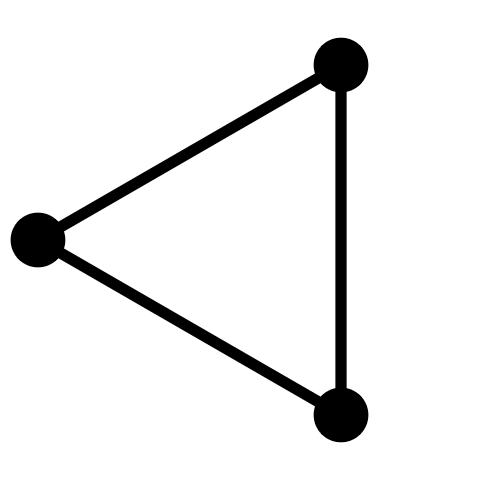
\includegraphics[width=.045\textwidth]{../FIGURES/FigMotif-Triangle} \end{tabular} 
  & 3.8 & 4.6 & 1.3 & -0.62\\ % & 0.69 \\ 
  \begin{tabular}{c} 
\includegraphics[width=.045\textwidth]{../FIGURES/FigMotif-Chain4} \end{tabular} 
  & 608.7 & 968.3 & 336.8 & -1.07 \\ % & 0.86 \\ 
  \begin{tabular}{c} 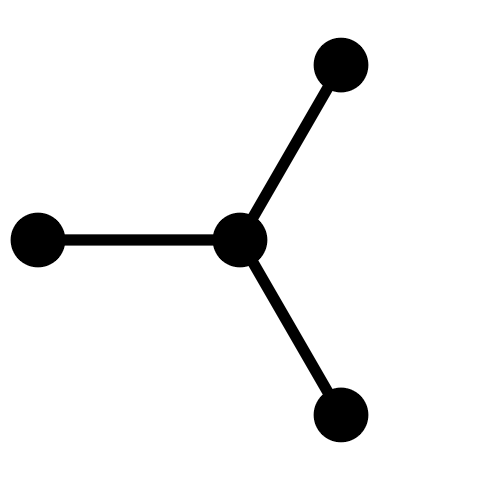
\includegraphics[width=.045\textwidth]{../FIGURES/FigMotif-Star3} \end{tabular}  
  & 279.8 & 428.9 & 154.0 & -0.97 \\ % & 0.83 \\ 
  \begin{tabular}{c} 
\includegraphics[width=.045\textwidth]{../FIGURES/FigMotif-Square} \end{tabular} 
  & 47.4 & 74.5 & 35.1 & -0.77 \\ % & 0.77 \\ 
  \begin{tabular}{c} 
\includegraphics[width=.045\textwidth]{../FIGURES/FigMotif-Whisker} \end{tabular} 
  & 270.5 & 397.0 & 177.0 & -0.71 \\ % & 0.75 \\ 
  \begin{tabular}{c} 
\includegraphics[width=.045\textwidth]{../FIGURES/FigMotif-SquareDiag} \end{tabular} 
  & 62.1 & 87.8 & 47.4 & -0.54 \\ % & 0.67 \\ 
  \begin{tabular}{c} 
\includegraphics[width=.045\textwidth]{../FIGURES/FigMotif-Clique4} \end{tabular} 
  & 6.5 & 8.8 & 5.4 & -0.43 \\ % & 0.61 \\ 
   \hline
\end{tabular}
$$

No specific structure seems to be exceptional wrt the model's expectations.

}

\backupend

%====================================================================
%====================================================================
\end{document}
%====================================================================
%====================================================================

  \begin{tabular}{cc}
    \begin{tabular}{p{.5\textwidth}}
    \end{tabular}
    & 
    \hspace{-.02\textwidth}
    \begin{tabular}{p{.5\textwidth}}
    \end{tabular}
  \end{tabular}

